\chapter{Anexos}

\section{Ejemplos de consultas} 
\label{sec:ejemplos}

En este anexo del trabajo sen va a mostrar algunas preguntas que se le pueden realizar al
sistema desarrollado a modo de ilustrar su
funcionamiento.

\section{Consultas REST}

Consulta realizada desde la documentación OpenAPI donde se consultas el total de defunciones
por Tuberculosis en España durante el año 2002 para los varones.
\FloatBarrier
\begin{figure}[h]
	\centering
	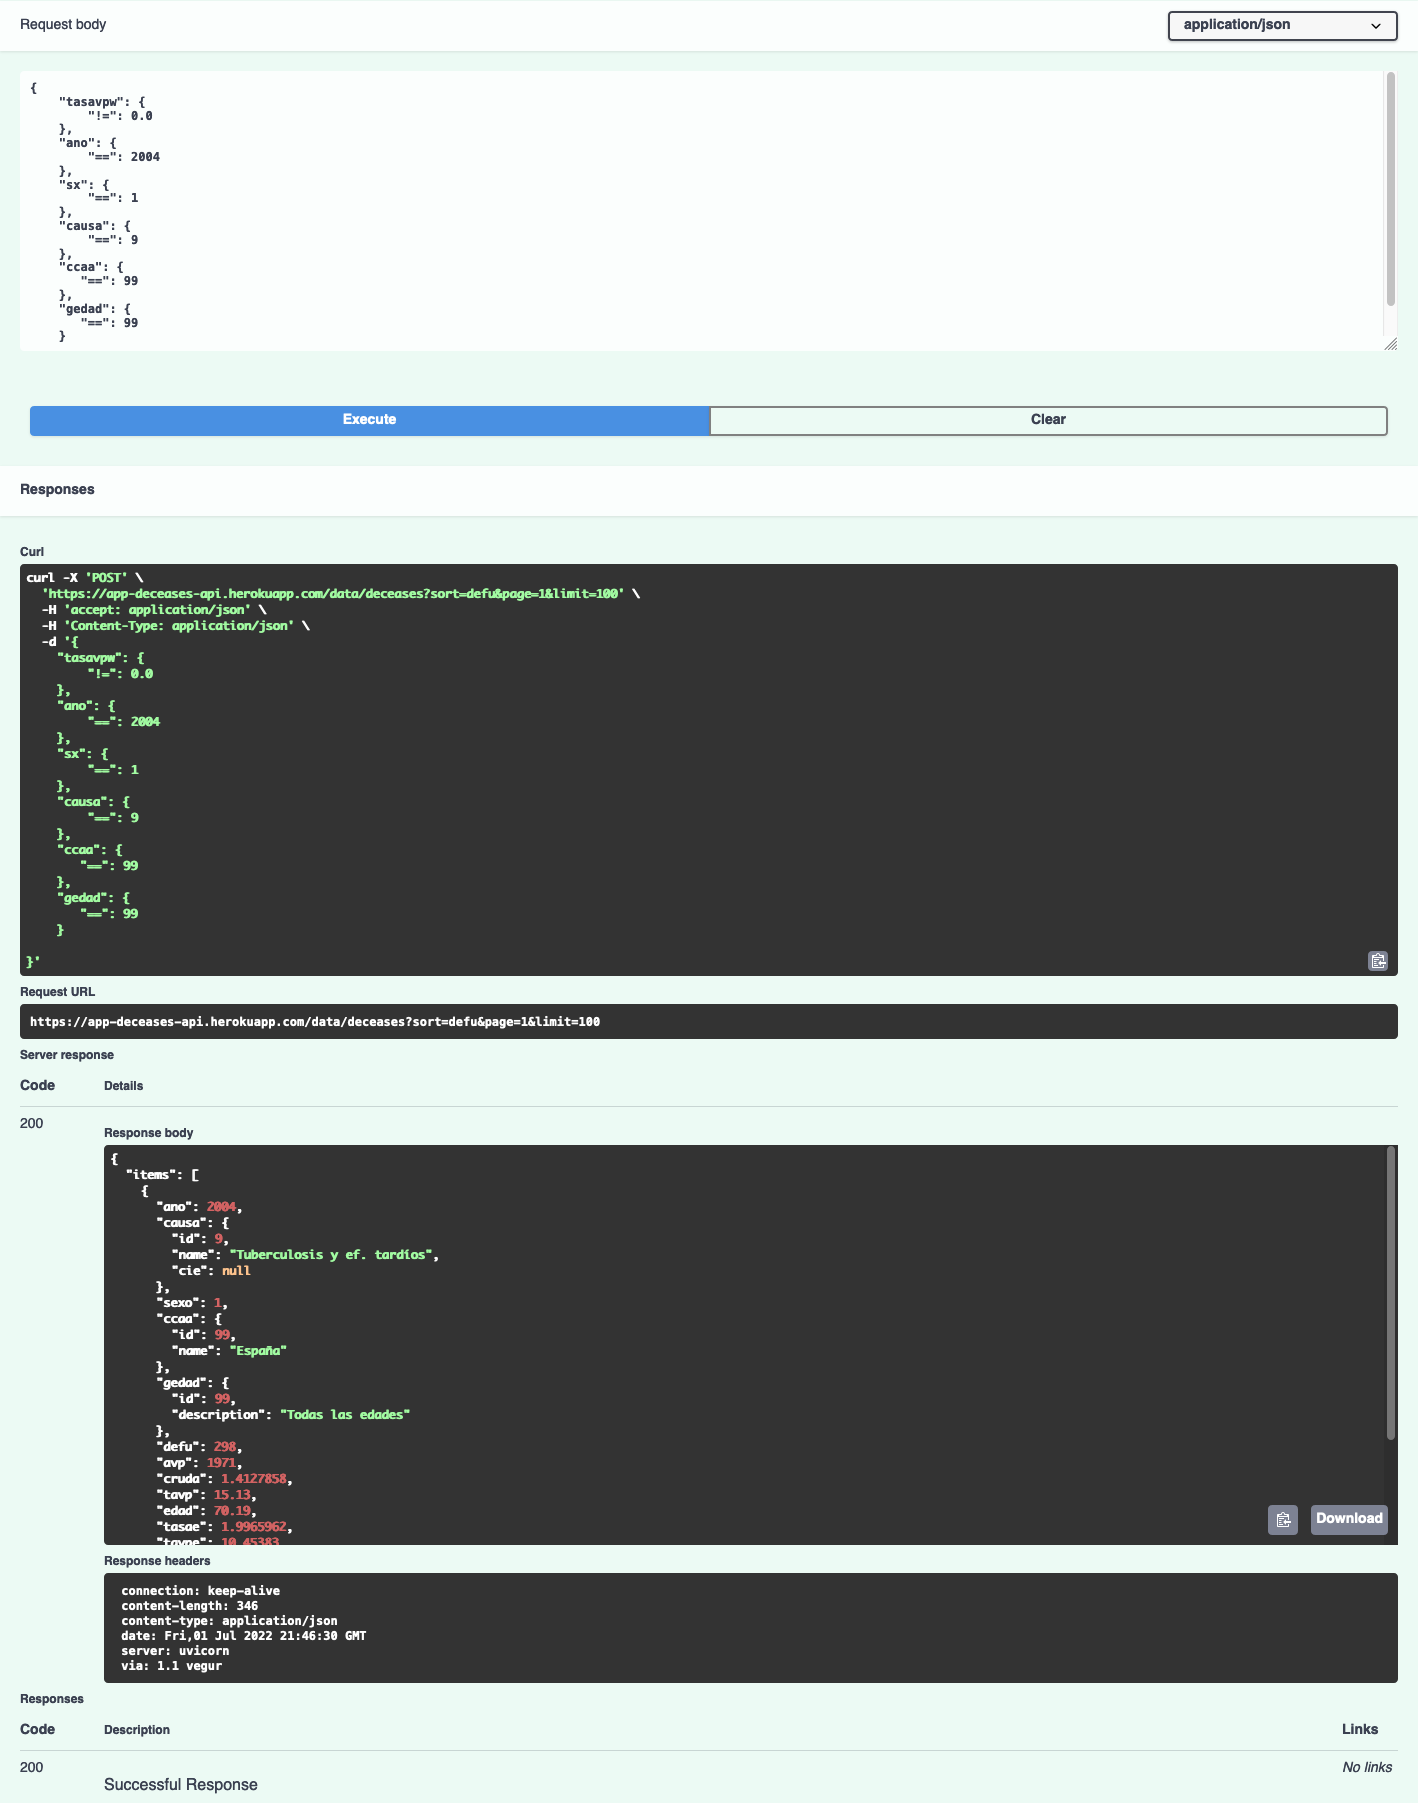
\includegraphics[width=\textwidth]{doc/logos/imgs/ejemplo1.png}
	\caption{ Consulta realizada a través de la documentación. }
\end{figure}
\FloatBarrier

Consulta realizada al manager de pronóstico sobre la evolución a 2 años de la causa de
muerte ``Paro cardíaco, muerte sin asistencia.''
Este manager a parte de ofrecer la gráfica también devuelve el conjunto de variables
estimadas.
\FloatBarrier
\begin{figure}[h]
	\centering
	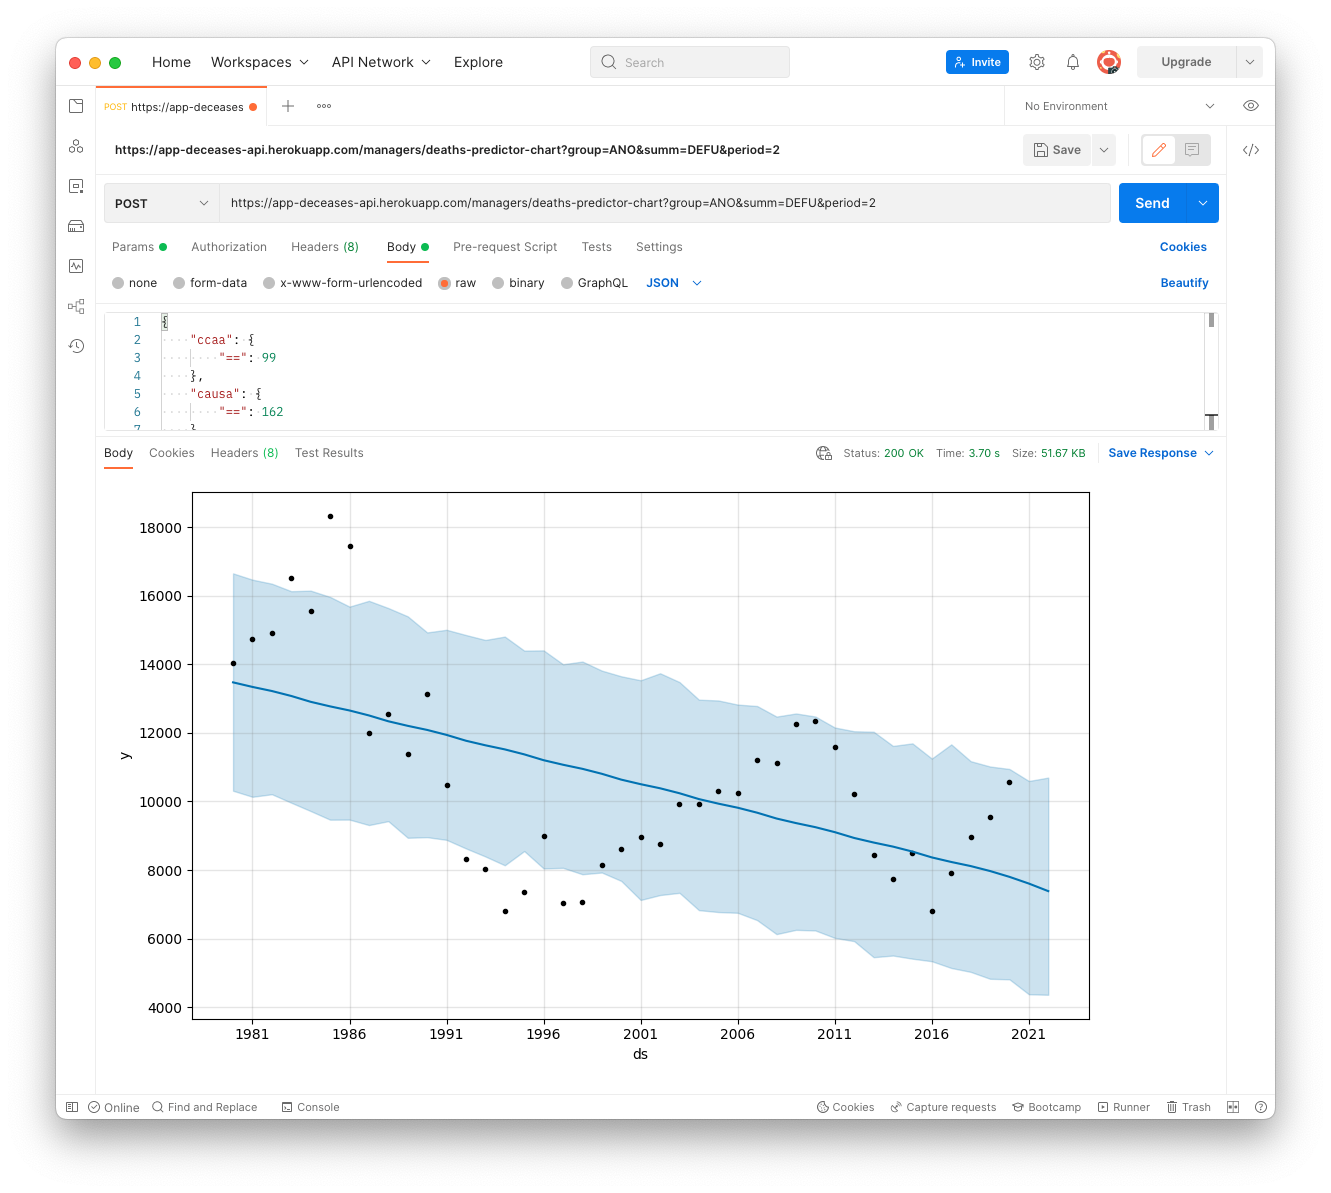
\includegraphics[width=\textwidth]{doc/logos/imgs/ejemplo2.png}
	\caption{ Consulta realizada a través de \href{https://www.postman.com/}{Postman}. }
\end{figure}
\FloatBarrier

\section{GraphiQL}

A continuación se puede apreciar el potencial del protocolo GraphQL donde podemos
proyectar únicamente los campos que son de nuestro interés y podemos obtener información
de distintos recursos en una única llamada.
\FloatBarrier
\begin{figure}[h]
	\centering
	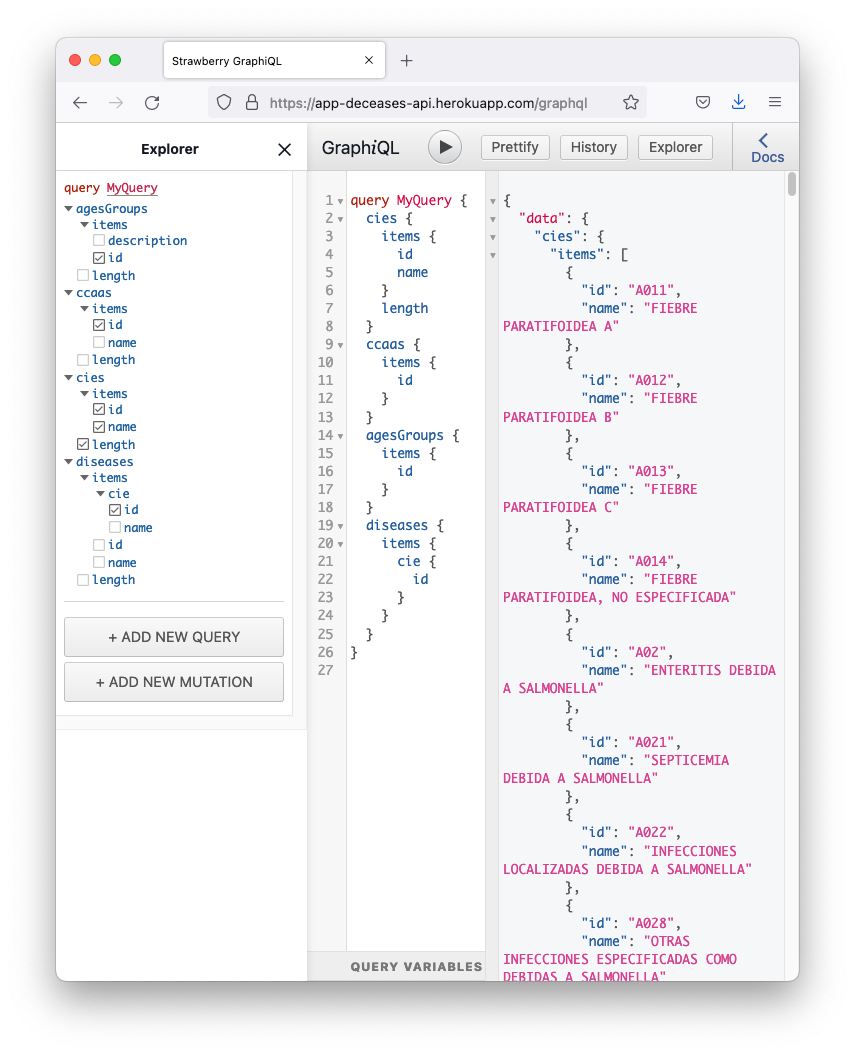
\includegraphics[width=\textwidth]{doc/logos/imgs/ejemplo3.png}
	\caption{ Consulta realizada a través de GraphiQL. }
\end{figure}
\FloatBarrier

Ejemplo de una operación de tipo mutación para obtener los distintos tipos de canceres que
clasifica el sistema con parámetros personalizados proyectados y paginados.
\FloatBarrier
\begin{figure}[h]
	\centering
	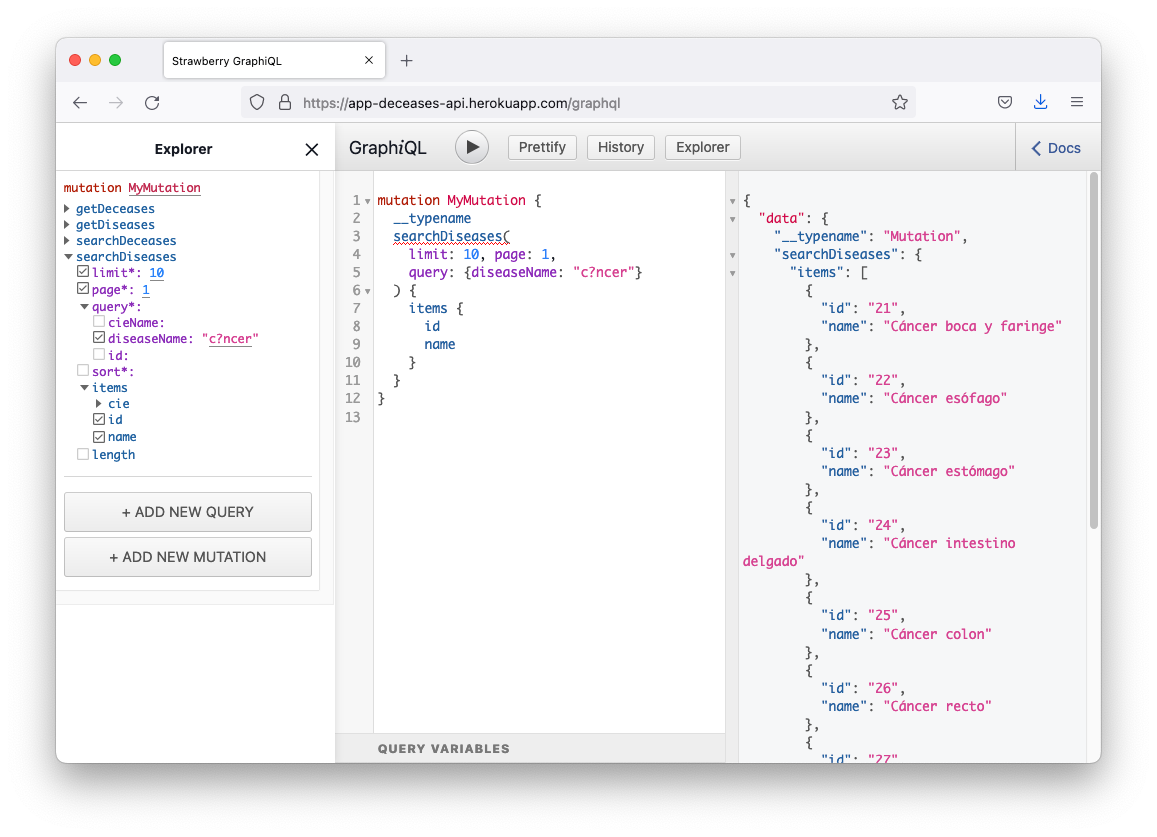
\includegraphics[width=\textwidth]{doc/logos/imgs/ejemplo4.png}
	\caption{ Mutación GraphQL. }
\end{figure}
\FloatBarrier

En esta consulta estamos realiando dos mutaciones donde solicitamos: la comunidad autónoma,
el número de defunciones y la edad media de la CCAA con más defunciones por Cáncer de boca
y faringe en 2018.
\FloatBarrier
\begin{figure}[h]
	\centering
	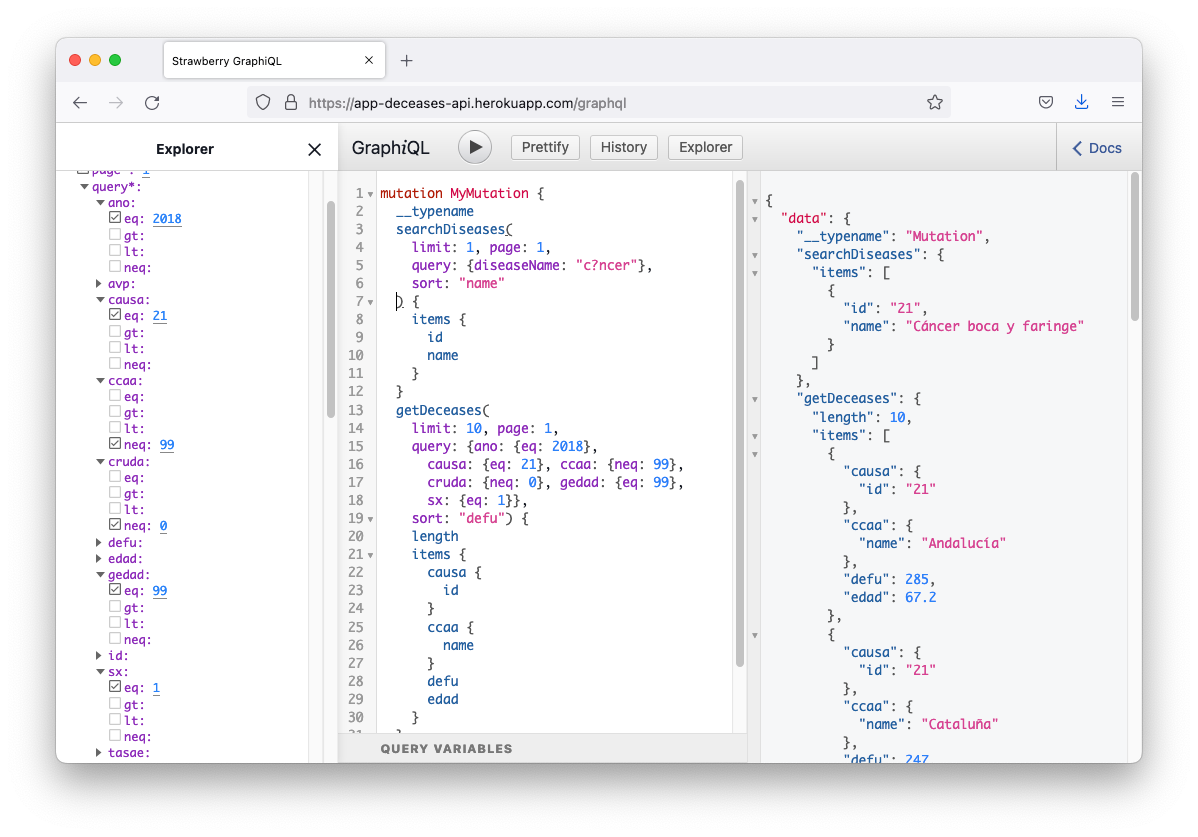
\includegraphics[width=\textwidth]{doc/logos/imgs/ejemplo5.png}
	\caption{ Mutación agrupadas GraphQL. }
\end{figure}
\FloatBarrier
